

% TRANSITION SLIDE
\begin{frame}[plain]
    \centering \hspace*{-1cm} \vspace*{-4cm}
        \begin{minipage}{0.8\textwidth}
            \centering
                {\usebeamerfont{section title}\usebeamercolor[fg]{section title}\LARGE
                    \textbf{Chapter 3:} \textit{\chapterthree}}
        \end{minipage}
        \vfill
\end{frame}


% CONTENT SLIDE
\begin{frame}{Colonization Resistance (CR)}
    \vspace*{-10mm} % move upwards
    \begin{minipage}[t][\usableheight][t]{\usablewidth}
        \begin{columns}[T]  
            \begin{column}{0.995\usablewidth} 
                \begin{block}{\tiny\cite{van_der_waaij_colonization_1971}}
                \centering \vspace*{2mm} % move down
                    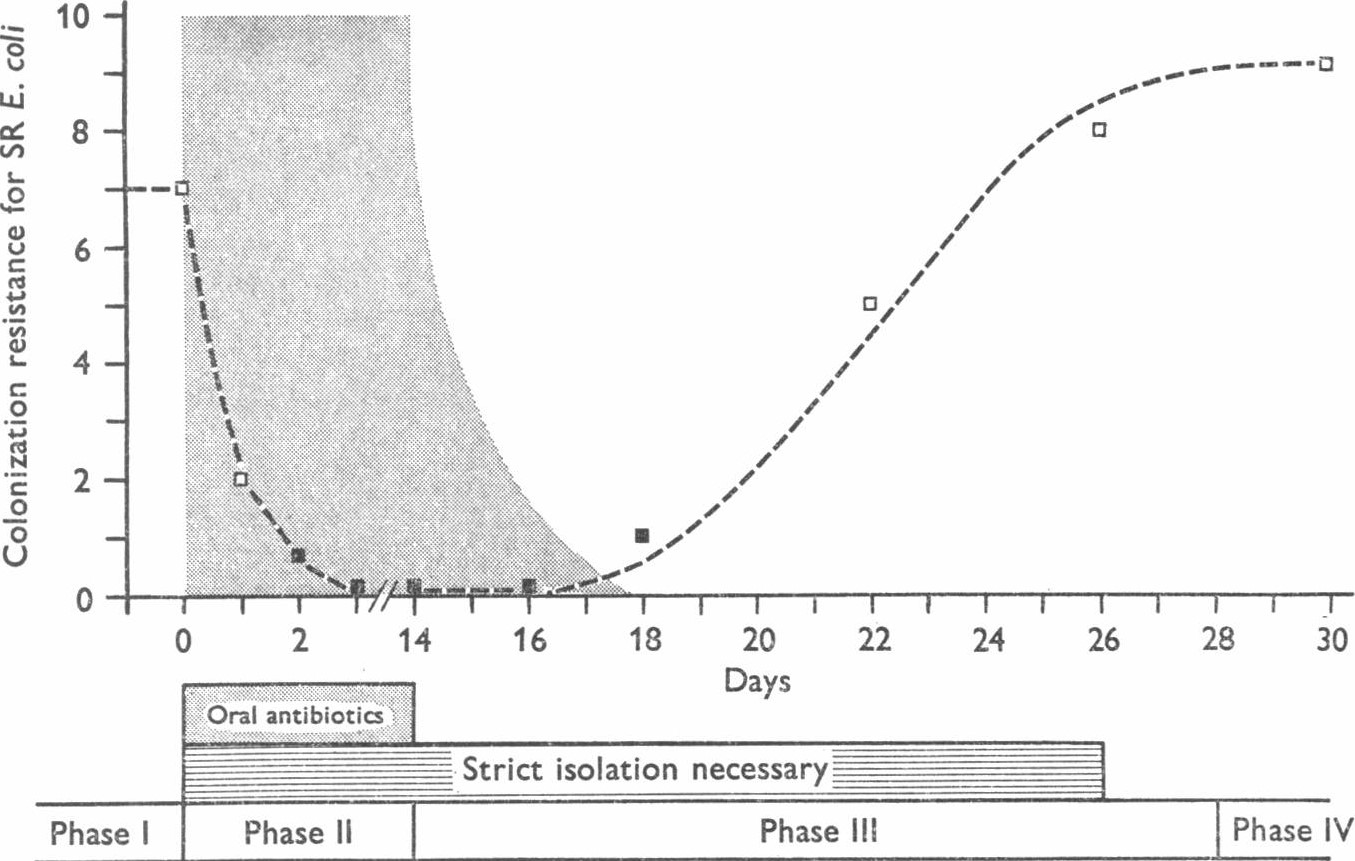
\includegraphics[
                        trim=0 0 0 0, clip,
                        width = 0.995\usablewidth, 
                        height=0.995\usableheight, % <-- Reduced to fit with block padding
                        keepaspectratio
                        ]{1971CR.jpg}
                \end{block}
            \end{column}
        \end{columns}
    \end{minipage}
\end{frame}